
\usepackage{fancyhdr}
\usepackage{lastpage}
\usepackage[utf8]{inputenc}

% Minted for syntax highliting
\usepackage{minted}
\usemintedstyle{tango}

% 
\usepackage[T1]{fontenc}
\usepackage{lmodern}

\usepackage{calc}
\usepackage{bytefield}

\usepackage{listings}
\usepackage{amsmath}

\usepackage{tikz}
\usetikzlibrary{automata,arrows,topaths,calc,positioning}
 
\usepackage{syntax}
\grammarindent=2cm


% Headers/footers styling
\pagestyle{fancy}
\fancyhf{}
\renewcommand{\headrulewidth}{0pt}

% Footer
\lfoot{ID1019}
\cfoot{KTH}
\rfoot{\thepage \hspace{1pt} / \pageref{LastPage}}

%\newcommand{\defaultpagestyle}{\thispagestyle{plain}}
\newcommand{\defaultpagestyle}{\thispagestyle{fancy}}



\usetikzlibrary{shapes.misc}


\title[ID1019 Concurrency]{Concurrency}

\author{Johan Montelius}
\institute{KTH}
\date{\semester}

\begin{document}

\begin{frame}
\titlepage
\end{frame}

\begin{frame}{What is concurrency?}

  \pause
  
  Concurrency: (the illusion of) happening at the same time.

  \vspace{20pt}\pause

  A property of the programming model.
  
  \vspace{20pt}\pause  

   Why would we want to do things concurrently?

\end{frame}


\begin{frame}[fragile]{concurrency vs parallelism}

  \begin{tikzpicture}
    \draw[->] (2,1) -- (2,8);
    \draw[->] (1,2) -- (12,2);    

    \node[anchor=south] at (7,1) {programing model};
    \node[anchor=south, rotate=90] at (0,5) {execution model};    
    
    \node[anchor=east] at (2,3) {sequential};
    \node[anchor=north] at (4,2) {sequential};

    \node[anchor=east] at (2,7) {parallel};
    \node[anchor=north] at (10,2) {concurrent};        
    
  \end{tikzpicture}


\end{frame}

\begin{frame}{concurrency models}

  \begin{itemize}
  \pause
  \item Shared memory:  modify a shared data structure
    \begin{itemize}
    \item C++/C
    \item Java
    \end{itemize} \pause
  \pause
  \item Message passing: processes send and receive messages
    \begin{itemize}
    \item Erlang/Exlixir 
    \item Go 
    \item Scala 
    \item Occam
    \item Rust
    \item Smalltalk
    \end{itemize}
  \end{itemize}

  \pause
  \vspace{40pt}{\em There are more, but these are the two large groups.}
\end{frame}

\begin{frame}{how do we send messages}

  \begin{itemize}
  \item Communicating Sequential Processes (CSP), messages are sent
    {\bf through channels}, a process can choose to read a message from one
    or more channels \pause
    \begin{itemize}
    \item Go, Occam, Rust
    \end{itemize}
    \pause
    
  \item Actor model, messages are sent {\bf to a process}, a process reads
    implicitly from its own channel \pause
    \begin{itemize}
    \item Smalltalk, Erlang/Elixir,  Scala 
    \end{itemize}    
  \end{itemize}
\end{frame}


\begin{frame}{actor model}

An actor:
\begin{itemize}
\item state: keeps a private state that can only be changed by the actor
\pause
\item receive: has one channel of incoming {\em messages}
\pause
\item execute: given a state and a received message, the actor can
\begin{itemize}
\pause
\item send: send a number of messages to other actors
\pause
\item spawn: create a number of new actors
\pause
\item transform: modify its state an continue, or terminate
\end{itemize}
\end{itemize}

\end{frame}


\begin{frame}{ordering of messages}

{\em Is the set of messages to an actor ordered?}

\pause\vspace{20pt}
{\em In what order should the messages be handled?}

\pause\vspace{20pt}
{\em The evaluation of a function is deterministic, how about the execution of an actor?}


\end{frame}

\begin{frame}{naming of actors}

{\em How can an actor direct a message to a specific actor?}

\pause\vspace{20pt}
{\em Do we have a global naming scheme?}

\pause\vspace{20pt}
{\em How do we find the identifier of an actor?}
     
\end{frame}



\begin{frame}{exceptions}

{\em What should we do if we're sending a message to an actor that has terminated?}

\pause\vspace{20pt}
{\em What if we're waiting for a message that will never be sent?}

\pause\vspace{20pt}
{\em Are sent messages guaranteed to arrive?}

\end{frame}


\begin{frame}{process identifier}

We introduce one additional data structure:
\pause\vspace{10pt}

$${\rm Structures} = \{\rm Process\ identifiers\} \cup {\rm Atoms} \cup \{\{s_1, s_2\} | s_i \in {\rm Structures}\}$$

\pause\vspace{20pt} 
{\em There is no term, nor pattern, that corresponds to an identifier.}
\end{frame}

\begin{frame}[fragile]{spawn}

  A new process is spawned by giving it a function to evaluate, \pause
  
  \vspace{10pt}\hspace{40pt}... the result is a process identifier (pid).

\pause\vspace{20pt}
\begin{verbatim}
  pid = spawn(fn() -> ... end)
\end{verbatim}
\pause\vspace{10pt}
or
\pause\vspace{10pt}
\begin{verbatim}
  pid = spawn(module, name, [arg, ...])
\end{verbatim}
\pause\vspace{10pt}
{\em In the later case, the function must be exported from the module.}

\end{frame}

\begin{frame}[fragile]{send}

Given a process identifier, an arbitrary data structure can be sent to the process.

\pause\vspace{10pt}

\begin{verbatim}
   send(pid, message)
\end{verbatim}

\pause\vspace{20pt}
{\em In Erlang this was written using an operator {\tt !},  often called ``bang''.}

\end{frame}

\begin{frame}{receive}

We extend expressions:

\pause\vspace{10pt}
\begin{code}
    <expression> ::=  & <receive expression> | ...
\end{code}
\pause\vspace{10pt}
\begin{code}
   <receive & expression> ::= \\
            & receive  do <clauses>  end
\end{code}
\pause\vspace{20pt}

{\em similar to case expressions}
\end{frame}

\begin{frame}[fragile]{example}

  \begin{verbatim}
def server(sum) do
  receive do
    {:add, x} ->
          server(sum + x)
    {sub, x} ->
          server(sum - x)
  end
end
\end{verbatim}

\end{frame}


\begin{frame}[fragile]{side effects}

In a {\em pure functional} program, the only effect of evaluating an
 expressions is the returned value \pause - not any more.

\pause
\begin{columns}[t]
  \begin{column}{0.5\linewidth}
\begin{verbatim}
     :
  bar(pid, 42)
  bar(pid, 32)
     :
\end{verbatim}
\pause\vspace{20pt}
\begin{verbatim}
def bar(pid, msg) do
    send(pid,{:hello, msg})
end
\end{verbatim}
  \end{column}
  \pause
  \begin{column}{0.5\linewidth}
\begin{verbatim}
     :
  x = foo(2)
  y = foo(2)
     :
\end{verbatim}
\pause\vspace{20pt}
\begin{verbatim}
def foo(x) do
   receive do
     {:hello, msg} -> msg + x
   end
end
\end{verbatim}
 \end{column}
\end{columns}  

\end{frame}


\begin{frame}[fragile]{Who am I?}

One more built-in function:

\pause\vspace{10pt}

\begin{verbatim}
    myPid = self()
\end{verbatim}

\end{frame}

\begin{frame}{few extensions}

Few extensions to the functional subset:
\pause\vspace{10pt}
\begin{itemize}
\pause\item pid: a process identifier as a data structure
\pause\item spawn: creating a process, returning a pid
\pause\item send: sending of messages to a pid
\pause\item receive: selective receive of messages
\pause\item self: the process identifier of the current process
\end{itemize}

\pause\vspace{10pt}
{\em All constructs can, apart from the receive statement, almost be given a functional interpretation.}

\pause\vspace{10pt}
{\em Our operational semantics does not give us any understanding of the execution.}

\end{frame}

\begin{frame}[fragile]{order of messages}

Message passing is: unreliable FIFO.

\pause\vspace{10pt}
\begin{verbatim}
           :
        send(pid, {:this, :is, :message, 1})
        send(pid, {:this, :is, :message, 2})
        send(pid, {:this, :is, :message, 3})
           :
\end{verbatim}

\pause What could be the result at the receiving end?

\pause\vspace{10pt}
{\em How many messages are lost in reality?} 

\end{frame}

\begin{frame}[fragile]{order of messages}

  \begin{columns}
    \begin{column}{0.5\textwidth}
Process one:
\begin{verbatim}
   :
send(pid, {:one, 1})
send(pid, {:one, 2})
   :
\end{verbatim}
    \end{column}
    \begin{column}{0.5\textwidth}
Process two:
\begin{verbatim}
   :
send(pid, {:two, 1})
send(pid, {:two, 2})
   :
\end{verbatim}
    \end{column}
  \end{columns}
  
\end{frame}

\begin{frame}[fragile]{selective receive}

\begin{verbatim}
def sum(s) do
  receive do
    {:add, x} -> sum(s + x)
    {:sub, x} -> sum(s - x)
    {:mul, x} -> sum(s * x)
  end
end
\end{verbatim}

\pause\vspace{10pt}

Assume we spawn a process given the expression {\tt fn() -> sum(10) end}, \pause and the sequence of messages in the queue is:

\vspace{10pt}
{\tt \{:sub, 4\}, \{:add, 10\}, \{:mul, 4\}, \{:mul, 2\}, \{:sub, 10\}}

\end{frame}



\begin{frame}[fragile]{selective receive}

\begin{columns}
 \begin{column}{0.5\linewidth}
\begin{verbatim}
def closed(s) do 
  receive 
    {:add, x} -> closed(s + x)
    :open -> open(s)
    :done -> {:ok, s}
  end
end
\end{verbatim}
 \end{column}
\pause
 \begin{column}{0.5\linewidth}
\begin{verbatim}
def open(s) do
  receive do
    {:mul, x} -> open(s * x)
    {:sub, x} -> open(s - x)
    :close -> closed(s)
  end
end
\end{verbatim}
\end{column}
\end{columns}


\pause\vspace{10pt}

Assume we spawn {\tt fn() -> closed(4) end} and the sequence of messages is:

\vspace{10pt}

{\tt \{:sub, 4\}, :open, \{:mul, 4\}, \{:add, 2\}, :close \{:add, 2\}, :done}

\pause\vspace{10pt}

In every receive expression we start from the beginning of the queue.

\end{frame}


\begin{frame}{implicit deferral}

{\em Selective receive}: we specify which messages we are willing to accept.

\pause\vspace{20pt}

{\em Implicit deferral}: messages that we do not explicitly receive, remain in the message queue.

\pause\vspace{20pt}
We coudl have chosen {\em fifo receive} i.e. messages must be received
in the order they have in the message queue (Actors model).

\pause\vspace{20pt}

We could have chosen {\em explicit deferral}, but then we would have to
state which messages that should be handled later.

\end{frame}

\begin{frame}{how to describe a processes}

  \begin{itemize}
  \item Finite state machine (FSM) : describing the states where messages determine transitions \pause 
  \item Sequence diagram : how processes interact, protcol definitions \pause
  \item Flow-based Programming (FBP) : architecture view of processes
  \item Domain Specific Language : describe the systems in a high level programing language \pause
  \item  ... 
  \end{itemize}
  
\end{frame}



\begin{frame}{finite state machine - FSM}


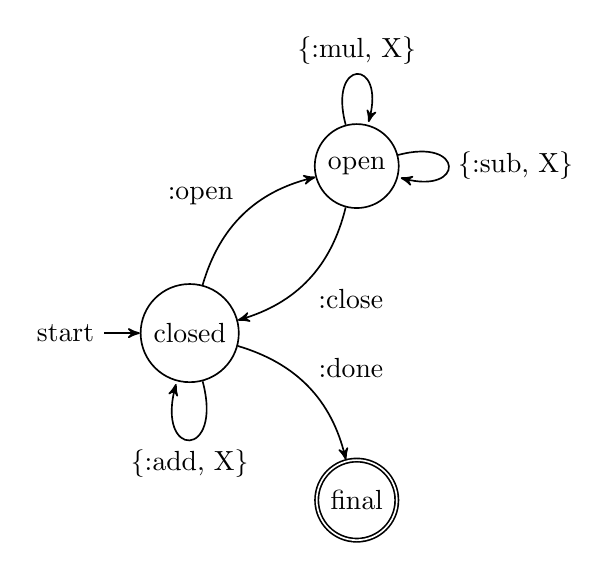
\begin{tikzpicture}[>=stealth', node distance=3cm, semithick, auto]
    \node[initial, state]            (closed)                              {closed};
    \node[state]                     (open)    [above right of=closed]     {open};
    \node[accepting, state]          (final)   [below right of=closed]     {final};

    \path[->]   (closed) edge       [bend left]     node      {:open}          (open)
                         edge       [loop below]    node      {\{:add, X\}}    (closed)
                         edge       [bend left]     node      {:done}          (final)
                (open)   edge       [loop above]    node      {\{:mul, X\}}    (open)
                         edge       [loop right]    node      {\{:sub, X\}}    (open)
                         edge       [bend left]     node      {:close}         (closed);
\end{tikzpicture}


\end{frame}


\begin{frame}{finite state machine - FSM}

Elixir receive statements are not a direct realization of a finite state machine.

\pause\vspace{10pt}

Messages that arrive too early in a finite state automata would give us an undefined state.

\pause\vspace{10pt}

The {\em implicit deferral} give us a very simple description of a
finite state machine where  messages are allowed to arrive too
early.


\end{frame}


\begin{frame}{sequence diagram}


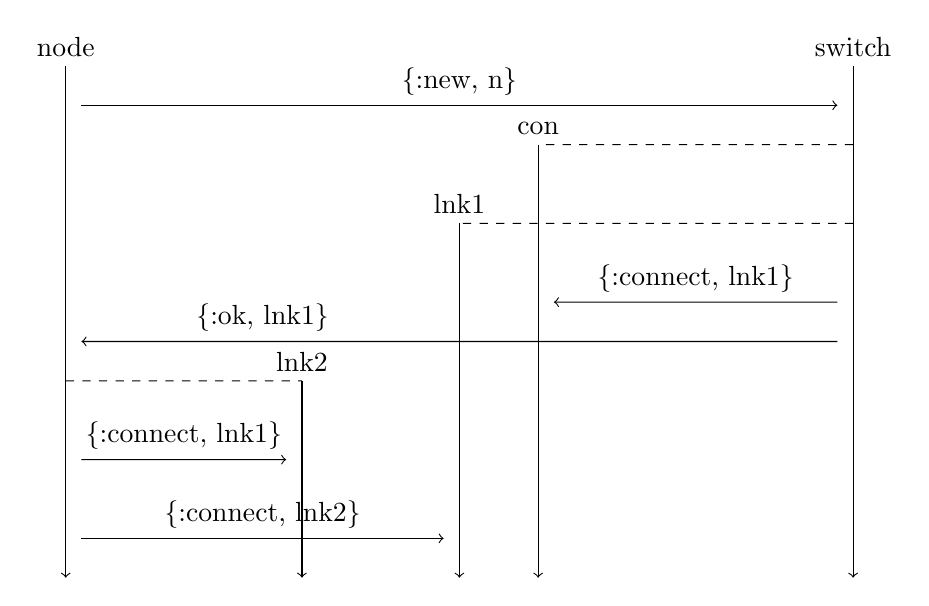
\begin{tikzpicture}

  \coordinate (n0) at (0,6);
  \coordinate (nn) at (0,-0.5);

  \coordinate (a0) at (3,2);
  \coordinate (an) at (3,-0.5);

  \coordinate (b0) at (5,4);
  \coordinate (bn) at (5,-0.5);

  \coordinate (c0) at (6,5);
  \coordinate (cn) at (6,-0.5);

  \coordinate (s0) at (10,6);
  \coordinate (sn) at (10,-0.5);

  \coordinate (n1) at ($(n0)+(0,-0.5)$);
  \coordinate (s1) at ($(s0)+(0,-0.5)$);

  \draw[->] (n0) to []  (nn);
  \draw[->] (s0) to []  (sn);

  \node[anchor=south] at (n0) {node};
  \node[anchor=south] at (s0) {switch};

  \pause

  \draw[->, shorten <=0.2cm, shorten >=0.2cm] (n1) -- node[midway, above] {\{:new, n\}} (s1);

  \pause

  \coordinate (s2) at ($(s1)+(0,-0.5)$);
  \coordinate (s3) at ($(s2)+(0,-1)$);

  \draw[dashed] (s2) -- (c0);

  \draw[dashed] (s3) -- (b0);

  \node[anchor=south] at (c0) {con};  
  \node[anchor=south] at (b0) {lnk1};  

  \draw[->] (c0) to []  (cn);
  \draw[->] (b0) to []  (bn);

\pause
  \coordinate (s4) at ($(s3)+(0,-1)$);
  \coordinate (c1) at ($(c0)+(0,-2)$);

  \draw[->, shorten <=0.2cm, shorten >=0.2cm] (s4) -- node[midway, above] {\{:connect, lnk1\}} (c1);

  \coordinate (s5) at ($(s4)+(0,-0.5)$);
  \coordinate (n2) at ($(n1)+(0,-3)$);

  \draw[->, shorten <=0.2cm, shorten >=0.2cm] (s5) -- node[near end, above] {\{:ok, lnk1\}} (n2);

  \draw[->] (a0) to []  (an);

  \node[anchor=south] at (a0) {lnk2};

  \coordinate (n3) at ($(n2)+(0,-0.5)$);
  \draw[dashed] (n3) -- (a0);

  \coordinate (n4) at ($(n3)+(0,-1)$);
  \coordinate (n5) at ($(n4)+(0,-1)$);
 
  \coordinate (a1) at ($(a0)+(0,-1)$);
  \coordinate (b1) at ($(b0)+(0,-4)$);

  \draw[->, shorten <=0.2cm, shorten >=0.2cm] (n4) -- node[midway, above] {\{:connect, lnk1\}} (a1);

  \draw[->, shorten <=0.2cm, shorten >=0.2cm] (n5) -- node[midway, above] {\{:connect, lnk2\}} (b1);

\end{tikzpicture}
  
\end{frame}

\begin{frame}{flow-based programming}

\begin{figure}
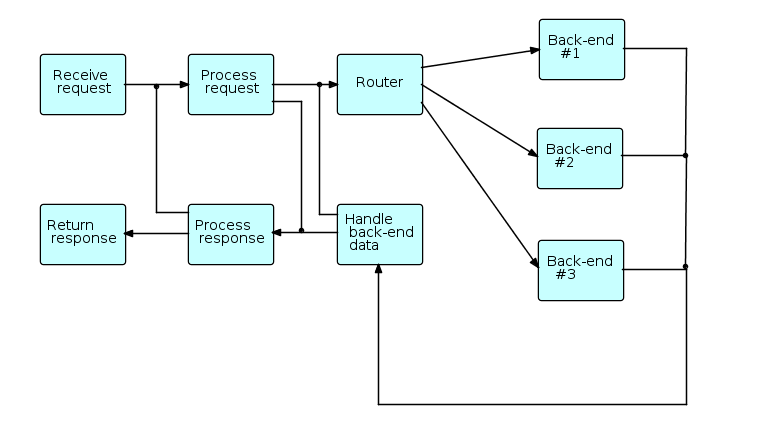
\includegraphics[scale=0.4]{fbp.png}
\caption{from J Paul Morrison www.jpaulmorrison.com}
\end{figure}
\end{frame}


\begin{frame}[fragile]{time to deliver}

\begin{columns}
   \begin{column}{.4\linewidth}
     \begin{block}{src/2}
\begin{verbatim}
def src(sink, frw) do
    send(sink, :a)
    send(frw, :b)
end
\end{verbatim}
      \end{block}
     \begin{block}{frw/2}
\begin{verbatim}
def frw(sink) do
   receive do
     msg -> send(sink,msg)
   end
end
\end{verbatim}
      \end{block}
    \end{column}
\pause
    \begin{column}{.6\linewidth}
      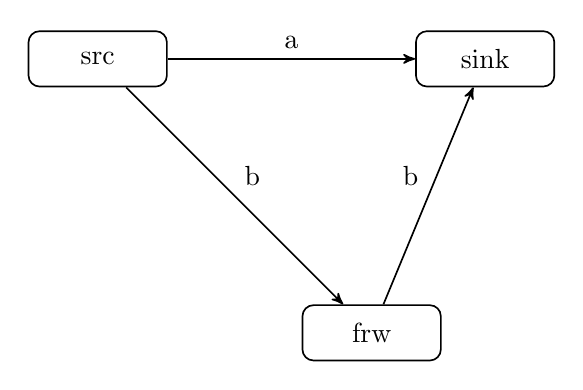
\begin{tikzpicture}[>=stealth', node distance=140pt, semithick, auto]

        \tikzstyle{fbp} = [rectangle, rounded corners, minimum width=50pt, minimum height=20pt,text centered, draw=black]        

        \node (src) [fbp] {src};
        \node (sink) [fbp, right of=src] {sink};
        \node (frw) [fbp, below right of=src] {frw};
        \path[->]  (src)   edge        node           {a}       (sink)
                          edge        node           {b}       (frw);
        \pause
        \path[->]  (frw)   edge        node           {b}       (sink);
\end{tikzpicture}
    \end{column}

  \end{columns}


\end{frame}
 
\begin{frame}[fragile]{example account}

\begin{columns}
   \begin{column}{.5\linewidth}
     \begin{verbatim}
def acc(saldo) do
  recieve do
     {:deposit, money} ->
        acc(saldo + money)
     {:withdraw, money} ->
        acc(saldo - money)
  end
end
     \end{verbatim}
   \end{column}
\pause
  \begin{column}{.5\linewidth}
     \begin{verbatim}
def doit() do
  acc = spawn(fn()->acc(0) end)
  send(acc, {:deposit, 20})
  send(acc, {:withdraw, 10})
  acc
end
     \end{verbatim}
   \end{column}
\end{columns}


\end{frame}

\begin{frame}[fragile]{example account}

\begin{columns}
   \begin{column}{.45\linewidth}
\begin{verbatim}
def acc(saldo) do
  recieve do
    {:deposit, money} ->
       acc(saldo + money)
    {:withdraw, money} ->
       acc(saldo - money)
    {:request, from} ->
       send(from, {:saldo, saldo})
       acc(saldo)
  end
end
\end{verbatim}
\end{column}
\pause
   \begin{column}{.45\linewidth}
\begin{verbatim}
def check(acc) do
  send(acc, {:request, self()})
  receive do
    {:saldo, saldo} ->
        saldo
  end
end
\end{verbatim}
\end{column}
\end{columns}
\end{frame}

\begin{frame}{summary}

\begin{itemize}
\item asynchronous: messages are sent and eventually (hopefully) delivered
\item FIFO: message delivery is ordered
\item selective receive: the receiver decides the order of handling messages
\item implicit deferral: messages remain in the queue until handled
\item diagrams: finite state machines, sequence diagrams, flow-based program
\end{itemize}

\end{frame}


\end{document}



